% Options for packages loaded elsewhere
\PassOptionsToPackage{unicode}{hyperref}
\PassOptionsToPackage{hyphens}{url}
\PassOptionsToPackage{dvipsnames,svgnames,x11names}{xcolor}
%
\documentclass[
  letterpaper,
  DIV=11,
  numbers=noendperiod]{scrartcl}

\usepackage{amsmath,amssymb}
\usepackage{iftex}
\ifPDFTeX
  \usepackage[T1]{fontenc}
  \usepackage[utf8]{inputenc}
  \usepackage{textcomp} % provide euro and other symbols
\else % if luatex or xetex
  \usepackage{unicode-math}
  \defaultfontfeatures{Scale=MatchLowercase}
  \defaultfontfeatures[\rmfamily]{Ligatures=TeX,Scale=1}
\fi
\usepackage{lmodern}
\ifPDFTeX\else  
    % xetex/luatex font selection
\fi
% Use upquote if available, for straight quotes in verbatim environments
\IfFileExists{upquote.sty}{\usepackage{upquote}}{}
\IfFileExists{microtype.sty}{% use microtype if available
  \usepackage[]{microtype}
  \UseMicrotypeSet[protrusion]{basicmath} % disable protrusion for tt fonts
}{}
\makeatletter
\@ifundefined{KOMAClassName}{% if non-KOMA class
  \IfFileExists{parskip.sty}{%
    \usepackage{parskip}
  }{% else
    \setlength{\parindent}{0pt}
    \setlength{\parskip}{6pt plus 2pt minus 1pt}}
}{% if KOMA class
  \KOMAoptions{parskip=half}}
\makeatother
\usepackage{xcolor}
\setlength{\emergencystretch}{3em} % prevent overfull lines
\setcounter{secnumdepth}{-\maxdimen} % remove section numbering
% Make \paragraph and \subparagraph free-standing
\ifx\paragraph\undefined\else
  \let\oldparagraph\paragraph
  \renewcommand{\paragraph}[1]{\oldparagraph{#1}\mbox{}}
\fi
\ifx\subparagraph\undefined\else
  \let\oldsubparagraph\subparagraph
  \renewcommand{\subparagraph}[1]{\oldsubparagraph{#1}\mbox{}}
\fi


\providecommand{\tightlist}{%
  \setlength{\itemsep}{0pt}\setlength{\parskip}{0pt}}\usepackage{longtable,booktabs,array}
\usepackage{calc} % for calculating minipage widths
% Correct order of tables after \paragraph or \subparagraph
\usepackage{etoolbox}
\makeatletter
\patchcmd\longtable{\par}{\if@noskipsec\mbox{}\fi\par}{}{}
\makeatother
% Allow footnotes in longtable head/foot
\IfFileExists{footnotehyper.sty}{\usepackage{footnotehyper}}{\usepackage{footnote}}
\makesavenoteenv{longtable}
\usepackage{graphicx}
\makeatletter
\def\maxwidth{\ifdim\Gin@nat@width>\linewidth\linewidth\else\Gin@nat@width\fi}
\def\maxheight{\ifdim\Gin@nat@height>\textheight\textheight\else\Gin@nat@height\fi}
\makeatother
% Scale images if necessary, so that they will not overflow the page
% margins by default, and it is still possible to overwrite the defaults
% using explicit options in \includegraphics[width, height, ...]{}
\setkeys{Gin}{width=\maxwidth,height=\maxheight,keepaspectratio}
% Set default figure placement to htbp
\makeatletter
\def\fps@figure{htbp}
\makeatother

\usepackage{booktabs}
\usepackage{longtable}
\usepackage{array}
\usepackage{multirow}
\usepackage{wrapfig}
\usepackage{float}
\usepackage{colortbl}
\usepackage{pdflscape}
\usepackage{tabu}
\usepackage{threeparttable}
\usepackage{threeparttablex}
\usepackage[normalem]{ulem}
\usepackage{makecell}
\usepackage{xcolor}
\usepackage[auth-lg]{authblk}
\KOMAoption{captions}{tableheading}
\makeatletter
\makeatother
\makeatletter
\makeatother
\makeatletter
\@ifpackageloaded{caption}{}{\usepackage{caption}}
\AtBeginDocument{%
\ifdefined\contentsname
  \renewcommand*\contentsname{Table of contents}
\else
  \newcommand\contentsname{Table of contents}
\fi
\ifdefined\listfigurename
  \renewcommand*\listfigurename{List of Figures}
\else
  \newcommand\listfigurename{List of Figures}
\fi
\ifdefined\listtablename
  \renewcommand*\listtablename{List of Tables}
\else
  \newcommand\listtablename{List of Tables}
\fi
\ifdefined\figurename
  \renewcommand*\figurename{Figure}
\else
  \newcommand\figurename{Figure}
\fi
\ifdefined\tablename
  \renewcommand*\tablename{Table}
\else
  \newcommand\tablename{Table}
\fi
}
\@ifpackageloaded{float}{}{\usepackage{float}}
\floatstyle{ruled}
\@ifundefined{c@chapter}{\newfloat{codelisting}{h}{lop}}{\newfloat{codelisting}{h}{lop}[chapter]}
\floatname{codelisting}{Listing}
\newcommand*\listoflistings{\listof{codelisting}{List of Listings}}
\makeatother
\makeatletter
\@ifpackageloaded{caption}{}{\usepackage{caption}}
\@ifpackageloaded{subcaption}{}{\usepackage{subcaption}}
\makeatother
\makeatletter
\@ifpackageloaded{tcolorbox}{}{\usepackage[skins,breakable]{tcolorbox}}
\makeatother
\makeatletter
\@ifundefined{shadecolor}{\definecolor{shadecolor}{rgb}{.97, .97, .97}}
\makeatother
\makeatletter
\makeatother
\makeatletter
\makeatother
\ifLuaTeX
  \usepackage{selnolig}  % disable illegal ligatures
\fi
\IfFileExists{bookmark.sty}{\usepackage{bookmark}}{\usepackage{hyperref}}
\IfFileExists{xurl.sty}{\usepackage{xurl}}{} % add URL line breaks if available
\urlstyle{same} % disable monospaced font for URLs
\hypersetup{
  pdftitle={Lista 2},
  pdfauthor={César Augusto Galvão - 19/0011572; Laiza Mendes - 20/0067028},
  colorlinks=true,
  linkcolor={blue},
  filecolor={Maroon},
  citecolor={Blue},
  urlcolor={Blue},
  pdfcreator={LaTeX via pandoc}}

\title{Lista 2}
\usepackage{etoolbox}
\makeatletter
\providecommand{\subtitle}[1]{% add subtitle to \maketitle
  \apptocmd{\@title}{\par {\large #1 \par}}{}{}
}
\makeatother
\subtitle{Modelos Lineares Generalizados - 2/2023}
\author{César Augusto Galvão - 19/0011572 \and Laiza Mendes -
20/0067028}
\date{}

\begin{document}
\maketitle
\ifdefined\Shaded\renewenvironment{Shaded}{\begin{tcolorbox}[enhanced, sharp corners, frame hidden, interior hidden, borderline west={3pt}{0pt}{shadecolor}, boxrule=0pt, breakable]}{\end{tcolorbox}}\fi

\renewcommand*\contentsname{Table of contents}
{
\hypersetup{linkcolor=}
\setcounter{tocdepth}{2}
\tableofcontents
}
\newpage{}

\hypertarget{questuxe3o-1}{%
\section{Questão 1}\label{questuxe3o-1}}

Considere os dados sobre a qualidade do vinho tinto, apresentados no
ficheiro \texttt{Q01-data.txt}. Ajuste o modelo de regressão linear
múltipla, e faça uma análise completa desses dados. Que conclusões você
tira dessa análise? (use 5\% de significância durantes as análises).

\hypertarget{a-proponha-algum-muxe9todo-para-resolver-o-problema-da-multicolinearidade-no-conjunto-de-dados}{%
\subsection{a) Proponha algum método para resolver o problema da
multicolinearidade no conjunto de
dados}\label{a-proponha-algum-muxe9todo-para-resolver-o-problema-da-multicolinearidade-no-conjunto-de-dados}}

\hypertarget{b-usando-algum-muxe9todo-de-seleuxe7uxe3o-de-variuxe1veis-obtenha-o-modelo-final-para-o-conjunto-de-dados}{%
\subsection{b) Usando algum método de seleção de variáveis, obtenha o
modelo final para o conjunto de
dados}\label{b-usando-algum-muxe9todo-de-seleuxe7uxe3o-de-variuxe1veis-obtenha-o-modelo-final-para-o-conjunto-de-dados}}

\hypertarget{c-apresente-a-tabela-de-anuxe1lise-de-variuxe2ncia-para-testar-a-significuxe2ncia-global-dos-coeficientes-do-modelo-final.-apresente-as-hipuxf3teses-de-teste-e-conclua.}{%
\subsection{c) Apresente a tabela de Análise de Variância para testar a
significância global dos coeficientes do modelo final. Apresente as
hipóteses de teste e
conclua.}\label{c-apresente-a-tabela-de-anuxe1lise-de-variuxe2ncia-para-testar-a-significuxe2ncia-global-dos-coeficientes-do-modelo-final.-apresente-as-hipuxf3teses-de-teste-e-conclua.}}

\hypertarget{d-com-base-no-modelo-obtido-no-item-anterior-fauxe7a-uma-anuxe1lise-de-resuxedduos-e-conclua.}{%
\subsection{d) Com base no modelo obtido no item anterior, faça uma
análise de resíduos e
conclua.}\label{d-com-base-no-modelo-obtido-no-item-anterior-fauxe7a-uma-anuxe1lise-de-resuxedduos-e-conclua.}}

\hypertarget{questuxe3o-2}{%
\section{Questão 2}\label{questuxe3o-2}}

Uma equipe de pesquisadores de saúde mental deseja comparar três métodos
de tratamento da depressão grave (A, B e C=referência). Eles também
gostariam de estudara relação entre idade e eficácia do tratamento, bem
como a interação (se houver) entre idade e tratamento. Cada elemento da
amostra aleatória simples de 36 pacientes, foi selecionado
aleatoriamente para receber o tratamento A, B ou C. Os dados obtidos
podem ser encontrados no ficheiro \texttt{Q02-data.txt}. A variável
dependente \(y\) é a eficácia do tratamento; as variáveis independentes
são: a idade do paciente no aniversário mais próximo e o tipo de
tratamento administrado (use 1\% de significância durantes as análises).

Uma amostra dos dados é exibida na tabela a seguir:

\begin{longtable*}{ccc}
\toprule
eficacia & idade & tratamento\\
\midrule
\endfirsthead
\multicolumn{3}{@{}l}{\textit{(continued)}}\\
\toprule
eficacia & idade & tratamento\\
\midrule
\endhead

\endfoot
\bottomrule
\endlastfoot
\cellcolor{gray!15}{56} & \cellcolor{gray!15}{21} & \cellcolor{gray!15}{A}\\
41 & 23 & B\\
\cellcolor{gray!15}{40} & \cellcolor{gray!15}{30} & \cellcolor{gray!15}{B}\\
28 & 19 & C\\
\cellcolor{gray!15}{55} & \cellcolor{gray!15}{28} & \cellcolor{gray!15}{A}\\
25 & 23 & C\\*
\end{longtable*}

\hypertarget{a-ajuste-um-modelo-de-regressuxe3o-linear-e-interprete-os-resultados-obtidos}{%
\subsection{a) Ajuste um modelo de regressão linear e interprete os
resultados
obtidos}\label{a-ajuste-um-modelo-de-regressuxe3o-linear-e-interprete-os-resultados-obtidos}}

Inicialmente, consideremos apenas um gráfico de dispersão entre a
variável resposta e a única variável numérica, Idade. É possível notar
uma relação que pode ou não ser linear, mas também há indícios de
heteroscedasticidade. As demais variáveis são dicotômicas, então não há
necessidade de se montar dispersões para elas.

Além disso, se segregamos a dispersão por grupos de tratamento, notamos
que pode ser preferível um modelo que considere comportamentos de cada
grupo separadamente.

\begin{figure}

{\centering 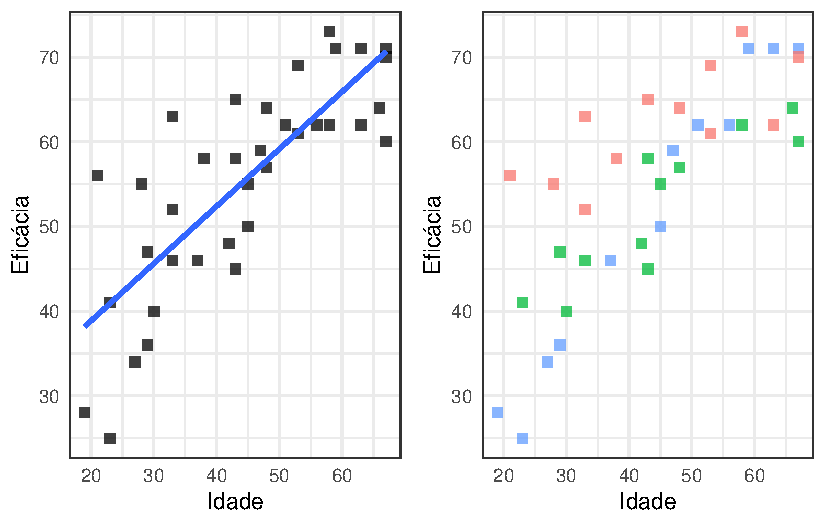
\includegraphics{lista2_files/figure-pdf/scatter-variaveis-1.pdf}

}

\end{figure}

Temos um potencial modelo de regressão linear que pode ou não conter
interações entre as variáveis, o qual pode ser expresso em sua forma
saturada, em que \(X_1\) é a variável idade e \(X_2\) a variável
tratamento

\begin{align}
  y_i = \beta_0 + \beta_1 \, x_{1i} + \beta_2 \, x_{2i} + \beta_3 \, x_{1i}\, x_{2i} + \varepsilon_i, \quad i = 1, 2, \dots, n
\end{align}

ou, de forma análoga, desmembrando \(X_2\) em variáveis \emph{dummy}
\(X_A\) e \(X_B\), indicadores da presença do tratamento \(A\) e \(B\),
ambas assumindo valor \(0\) quando se trata do tratamento \(C\)

\begin{align}
  y_i = \beta_0 + \beta_1 \, x_{1i} + \beta_2 \, x_{Ai} + \beta_3 \, x_{Bi} + \beta_4 \, x_{1i} \, x_{Ai} + \beta_5 \, x_{1i} \, x_{Bi} + \varepsilon_i. \label{modelo_dummy}
\end{align}

Se simplesmente ajustamos um modelo de regressão linear -- sem os termos
de interação -- utilizando (\ref{modelo_dummy}) como referência na
função \texttt{lm()}, obtemos os seguintes resultados:

\begin{longtable}[t]{lcccc}
\caption{Modelo de regressão linear para tratamentos sem interação com idade sobre eficácia}\\
\toprule
Coeficiente & Estimativa & EP & Estatística t & p-valor\\
\midrule
\endfirsthead
\caption[]{Modelo de regressão linear para tratamentos sem interação com idade sobre eficácia \textit{(continued)}}\\
\toprule
Coeficiente & Estimativa & EP & Estatística t & p-valor\\
\midrule
\endhead

\endfoot
\bottomrule
\endlastfoot
\cellcolor{gray!15}{(Intercept)} & \cellcolor{gray!15}{22.291} & \cellcolor{gray!15}{3.505} & \cellcolor{gray!15}{6.359} & \cellcolor{gray!15}{0.000}\\
idade & 0.664 & 0.070 & 9.522 & 0.000\\
\cellcolor{gray!15}{A} & \cellcolor{gray!15}{10.253} & \cellcolor{gray!15}{2.465} & \cellcolor{gray!15}{4.159} & \cellcolor{gray!15}{0.000}\\
B & 0.445 & 2.464 & 0.181 & 0.858\\*
\end{longtable}

Ou seja, se considerarmos independentemente idade, tratamento A e
tratamento B, podemos considerar que:

\begin{itemize}
\tightlist
\item
  Há uma linha de base na eficácia de aproximadamente 22.3, i.e.~sob o
  tratamento C;
\item
  A eficácia base para o tratamento A é de 32.3;
\item
  A eficácia base para o tratamento B é de 22.75 -- mas poderíamos
  desconsiderar este coeficiente, se nos guiarmos pelo p-valor;
\item
  Cada ano a mais de vida incrementa a eficácia em 0.644.
\end{itemize}

É possível considerar que um tamanho de amostra pequeno tenha grande
influência sobre a significância de \(H_0: \beta_3 = 0\) do modelo. No
entanto, trata-se de um fenômeno para o qual o tratamento pode estar
estreitamente associado à idade, caso em que teríamos que considerar o
modelo (\ref{modelo_dummy}) por completo.

\hypertarget{b-obtenha-a-tabela-anova-para-o-modelo-obtido-no-item-a-e-interprete-os-resultados}{%
\subsection{b) Obtenha a tabela ANOVA para o modelo obtido no item (a) e
interprete os
resultados}\label{b-obtenha-a-tabela-anova-para-o-modelo-obtido-no-item-a-e-interprete-os-resultados}}

Se montarmos uma tabela de Análise de Variância para o modelo de
regressão linear ajustado, obtemos os resultados a seguir:

\begin{longtable}[t]{lccccl}
\caption{Tabela ANOVA para o modelo linear sem interações}\\
\toprule
Fonte de Var. & g.l. & SQ & QM & F & p-valor\\
\midrule
\endfirsthead
\caption[]{Tabela ANOVA para o modelo linear sem interações \textit{(continued)}}\\
\toprule
Fonte de Var. & g.l. & SQ & QM & F & p-valor\\
\midrule
\endhead

\endfoot
\bottomrule
\endlastfoot
\cellcolor{gray!15}{idade} & \cellcolor{gray!15}{1} & \cellcolor{gray!15}{3424.432} & \cellcolor{gray!15}{3424.432} & \cellcolor{gray!15}{94.015} & \cellcolor{gray!15}{0.000}\\
A & 1 & 803.804 & 803.804 & 22.068 & 0.000\\
\cellcolor{gray!15}{B} & \cellcolor{gray!15}{1} & \cellcolor{gray!15}{1.189} & \cellcolor{gray!15}{1.189} & \cellcolor{gray!15}{0.033} & \cellcolor{gray!15}{0.858}\\
Residuals & 32 & 1165.575 & 36.424 & NA & NA\\*
\end{longtable}

Nota-se que a maioria da variância explicada pelo modelo está associada
à variável idade, enquanto a soma de quadrados das variáveis de
tratamento juntas não superam a soma de quadrados dos resíduos.

Se conjugarmos os resultados deste item com os do item a) vemos que
isoladamente apenas idade, e interessantemente apenas o tratamento A,
parecem ser variáveis que realmente contribuem para a explicação do
fenômeno.

\hypertarget{c-considere-a-possibilidade-de-incluir-a-interauxe7uxe3o-entre-as-varuxe1veis-independentes}{%
\subsection{c) Considere a possibilidade de incluir a interação entre as
varáveis
independentes}\label{c-considere-a-possibilidade-de-incluir-a-interauxe7uxe3o-entre-as-varuxe1veis-independentes}}

\hypertarget{i-lista-de-todos-os-submodelos-possuxedveis}{%
\subsubsection{i) Lista de todos os submodelos
possíveis}\label{i-lista-de-todos-os-submodelos-possuxedveis}}

A partir do modelo (\ref{modelo_dummy}), construimos todos os possíveis
submodelos. Considerando que temos três covariáveis e dois termos de
interação, temos \(\sum\limits_{n = 1}^5\binom{6}{n} = 62\) modelos

\begin{enumerate}
  \item $y_i = \beta_0 + \varepsilon_i$
  \item $y_i = \beta_1 \, x_{1i} + \varepsilon_i$
  \item $y_i = \beta_2 \, x_{Ai} + \varepsilon_i$
  \item $y_i = \beta_3 \, x_{Bi} + \varepsilon_i$
  \item $y_i = \beta_4 \, x_{1i} \, x_{Ai} + \varepsilon_i$
  \item $y_i = \beta_5 \, x_{1i} \, x_{Bi} + \varepsilon_i$
  
 
  \item $y_i = \beta_0 + \beta_1 \, x_{1i} + \varepsilon_i$
  \item $y_i = \beta_0 + \beta_2 \, x_{Ai} + \varepsilon_i$
  \item $y_i = \beta_0 + \beta_3 \, x_{Bi} + \varepsilon_i$
  \item $y_i = \beta_0 + \beta_4 \, x_{1i} \, x_{Ai} + \varepsilon_i$
  \item $y_i = \beta_0 + \beta_5 \, x_{1i} \, x_{Bi} + \varepsilon_i$
  \item $y_i = \beta_1 \, x_{1i} + \beta_2 \, x_{Ai} + \varepsilon_i$
  \item $y_i = \beta_1 \, x_{1i} + \beta_3 \, x_{Bi} + \varepsilon_i$
  \item $y_i = \beta_1 \, x_{1i} + \beta_4 \, x_{1i} \, x_{Ai} + \varepsilon_i$
  \item $y_i =  \beta_1 \, x_{1i} + \beta_5 \, x_{1i} \, x_{Bi} + \varepsilon_i$
  \item $y_i = \beta_2 \, x_{Ai} + \beta_3 \, x_{Bi}+ \varepsilon_i$
  \item $y_i = \beta_2 \, x_{Ai} + \beta_4 \, x_{1i} \, x_{Ai} + \varepsilon_i$
  \item $y_i = \beta_2 \, x_{Ai} + \beta_5 \, x_{1i} \, x_{Bi} + \varepsilon_i$
  \item $y_i = \beta_3 \, x_{Bi} + \beta_4 \, x_{1i} \, x_{Ai} + \varepsilon_i$
  \item $y_i = \beta_3 \, x_{Bi} \beta_5 \, x_{1i} \, x_{Bi} + \varepsilon_i$
  \item $y_i = \beta_4 \, x_{1i} \, x_{Ai} + \beta_5 \, x_{1i} \, x_{Bi} + \varepsilon_i$
  
  

  \item $y_i = \beta_0 + \beta_1 \, x_{1i} + \beta_2 \, x_{Ai} + \varepsilon_i$
  \item $y_i = \beta_0 + \beta_1 \, x_{1i} + \beta_3 \, x_{Bi} + \varepsilon_i$
  \item $y_i = \beta_0 + \beta_1 \, x_{1i} + \beta_4 \, x_{1i} \, x_{Ai} + \varepsilon_i$
  \item $y_i = \beta_0 + \beta_1 \, x_{1i} + \beta_5 \, x_{1i} \, x_{Bi} + \varepsilon_i$
  \item $y_i = \beta_0 + \beta_2 \, x_{Ai} + \beta_3 \, x_{Bi} + \varepsilon_i$
  \item $y_i = \beta_0 + \beta_2 \, x_{Ai} + \beta_4 \, x_{1i} \, x_{Ai} +  \varepsilon_i$
  \item $y_i = \beta_0 + \beta_2 \, x_{Ai} + \beta_5 \, x_{1i} \, x_{Bi} + \varepsilon_i$
  \item $y_i = \beta_0 + \beta_3 \, x_{Bi} + \beta_4 \, x_{1i} \, x_{Ai} +  \varepsilon_i$
  \item $y_i = \beta_0 + \beta_3 \, x_{Bi} + \beta_5 \, x_{1i} \, x_{Bi} + \varepsilon_i$
  \item $y_i = \beta_0 + \beta_4 \, x_{1i} \, x_{Ai} + \beta_5 \, x_{1i} \, x_{Bi} + \varepsilon_i$
  \item $y_i = \beta_1 \, x_{1i} + \beta_2 \, x_{Ai} + \beta_3 \, x_{Bi} + \varepsilon_i$
  \item $y_i = \beta_1 \, x_{1i} + \beta_2 \, x_{Ai} + \beta_4 \, x_{1i} \, x_{Ai} + \varepsilon_i$
  \item $y_i = \beta_1 \, x_{1i} + \beta_2 \, x_{Ai} + \beta_5 \, x_{1i} \, x_{Bi} + \varepsilon_i$
  \item $y_i = \beta_1 \, x_{1i} + \beta_3 \, x_{Bi} + \beta_4 \, x_{1i} \, x_{Ai} + \varepsilon_i$
  \item $y_i = \beta_1 \, x_{1i} + \beta_3 \, x_{Bi} + \beta_5 \, x_{1i} \, x_{Bi} + \varepsilon_i$
  \item $y_i = \beta_1 \, x_{1i} + \beta_4 \, x_{1i} \, x_{Ai} + \beta_5 \, x_{1i} \, x_{Bi} + \varepsilon_i$
  \item $y_i = \beta_2 \, x_{Ai} + \beta_3 \, x_{Bi} + \beta_4 \, x_{1i} \, x_{Ai} + \varepsilon_i$
  \item $y_i = \beta_2 \, x_{Ai} + \beta_3 \, x_{Bi} + \beta_5 \, x_{1i} \, x_{Bi} + \varepsilon_i$
  \item $y_i = \beta_2 \, x_{Ai} + \beta_4 \, x_{1i} \, x_{Ai} + \beta_5 \, x_{1i} \, x_{Bi} + \varepsilon_i$
  \item $y_i = \beta_3 \, x_{Bi} + \beta_4 \, x_{1i} \, x_{Ai} + \beta_5 \, x_{1i} \, x_{Bi} + \varepsilon_i$
  

 
  \item $y_i = \beta_0 + \beta_1 \, x_{1i} + \beta_2 \, x_{Ai} + \beta_3 \, x_{Bi} + \varepsilon_i$
  \item $y_i = \beta_0 + \beta_1 \, x_{1i} + \beta_2 \, x_{Ai} + \beta_4 \, x_{1i} \, x_{Ai} + \varepsilon_i$
  \item $y_i = \beta_0 + \beta_1 \, x_{1i} + \beta_2 + \beta_5 \, x_{1i} \, x_{Bi} + \varepsilon_i$
  \item $y_i = \beta_0 + \beta_1 \, x_{1i} + \beta_3 \, x_{Bi} + \beta_4 \, x_{1i} \, x_{Ai} + \varepsilon_i$
  \item $y_i = \beta_0 + \beta_1 \, x_{1i} + \beta_3 \, x_{Bi} + \beta_5 \, x_{1i} \, x_{Bi} + \varepsilon_i$
  \item $y_i = \beta_0 + \beta_1 \, x_{1i} + \beta_4 \, x_{1i} \, x_{Ai} + \beta_5 \, x_{1i} \, x_{Bi} + \varepsilon_i$
  
  \item $y_i = \beta_0 + \beta_2 \, x_{Ai} + \beta_3 \, x_{Bi} + \beta_4 \, x_{1i} \, x_{Ai} + \varepsilon_i$
  \item $y_i = \beta_0 + \beta_2 \, x_{Ai} + \beta_3 \, x_{Bi} + \beta_5 \, x_{1i} \, x_{Bi} + \varepsilon_i$
  \item $y_i = \beta_0 + \beta_2 \, x_{Ai} + \beta_4 \, x_{1i} \, x_{Ai} + \beta_5 \, x_{1i} \, x_{Bi} + \varepsilon_i$
  \item $y_i = \beta_0 + \beta_3 \, x_{Bi} + \beta_4 \, x_{1i} \, x_{Ai} + \beta_5 \, x_{1i} \, x_{Bi} + \varepsilon_i$
  
  \item $y_i = \beta_1 \, x_{1i} + \beta_2 \, x_{Ai} + \beta_3 \, x_{Bi} + \beta_4 \, x_{1i} \, x_{Ai} + \varepsilon_i$
  \item $y_i = \beta_1 \, x_{1i} + \beta_2 \, x_{Ai} + \beta_3 \, x_{Bi} + \beta_5 \, x_{1i} \, x_{Bi} + \varepsilon_i$
  \item $y_i = \beta_1 \, x_{1i} + \beta_2 \, x_{Ai} + \beta_4 \, x_{1i} \, x_{Ai} + \beta_5 \, x_{1i} \, x_{Bi} + \varepsilon_i$
  \item $y_i = \beta_1 \, x_{1i} + \beta_3 \, x_{Bi} + \beta_4 \, x_{1i} \, x_{Ai} + \beta_5 \, x_{1i} \, x_{Bi} + \varepsilon_i$
  
  \item $y_i = \beta_2 \, x_{Ai} + \beta_3 \, x_{Bi} + \beta_4 \, x_{1i} \, x_{Ai} + \beta_5 \, x_{1i} \, x_{Bi} + \varepsilon_i$
  
  \item $y_i = \beta_1 \, x_{1i} + \beta_2 \, x_{Ai} + \beta_3 \, x_{Bi} + \beta_4 \, x_{1i} \, x_{Ai} + \beta_5 \, x_{1i} \, x_{Bi} + \varepsilon_i$
  
  \item $y_i = \beta_0 + \beta_2 \, x_{Ai} + \beta_3 \, x_{Bi} + \beta_4 \, x_{1i} \, x_{Ai} + \beta_5 \, x_{1i} \, x_{Bi} + \varepsilon_i$
  \item $y_i = \beta_0 + \beta_1 \, x_{1i} + \beta_3 \, x_{Bi} + \beta_4 \, x_{1i} \, x_{Ai} + \beta_5 \, x_{1i} \, x_{Bi} + \varepsilon_i$
  \item $y_i = \beta_0 + \beta_1 \, x_{1i} + \beta_2 \, x_{Ai} + \beta_4 \, x_{1i} \, x_{Ai} + \beta_5 \, x_{1i} \, x_{Bi} + \varepsilon_i$
  \item $y_i = \beta_0 + \beta_1 \, x_{1i} + \beta_2 \, x_{Ai} + \beta_3 \, x_{Bi} + \beta_5 \, x_{1i} \, x_{Bi} + \varepsilon_i$
  \item $y_i = \beta_0 + \beta_1 \, x_{1i} + \beta_2 \, x_{Ai} + \beta_3 \, x_{Bi} + \beta_4 \, x_{1i} \, x_{Ai} + \varepsilon_i$
\end{enumerate}

\hypertarget{ii-interpretauxe7uxe3o-de-coeficientes-de-regressuxe3o-de-fatores-de-interauxe7uxe3o}{%
\subsubsection{ii) Interpretação de coeficientes de regressão de fatores
de
interação}\label{ii-interpretauxe7uxe3o-de-coeficientes-de-regressuxe3o-de-fatores-de-interauxe7uxe3o}}

Agora experimentamos ajustar exatamente o modelo (\ref{modelo_dummy}) e,
conforme suspeitas, verificamos que não apenas agora o coeficiente
\(\beta_3\), correspondente ao tratamento B, é significativamente
diferente de zero, como a interação dos tratamentos também o é.

\begin{longtable}[t]{lcccc}
\caption{Modelo de regressão linear para tratamentos com interação com idade sobre eficácia}\\
\toprule
Coeficiente & Estimativa & EP & Estatística t & p-valor\\
\midrule
\endfirsthead
\caption[]{Modelo de regressão linear para tratamentos com interação com idade sobre eficácia \textit{(continued)}}\\
\toprule
Coeficiente & Estimativa & EP & Estatística t & p-valor\\
\midrule
\endhead

\endfoot
\bottomrule
\endlastfoot
\cellcolor{gray!15}{(Intercept)} & \cellcolor{gray!15}{6.211} & \cellcolor{gray!15}{3.350} & \cellcolor{gray!15}{1.854} & \cellcolor{gray!15}{0.074}\\
idade & 1.033 & 0.072 & 14.288 & 0.000\\
\cellcolor{gray!15}{A} & \cellcolor{gray!15}{41.304} & \cellcolor{gray!15}{5.085} & \cellcolor{gray!15}{8.124} & \cellcolor{gray!15}{0.000}\\
B & 22.707 & 5.091 & 4.460 & 0.000\\
\cellcolor{gray!15}{idade:A} & \cellcolor{gray!15}{-0.703} & \cellcolor{gray!15}{0.109} & \cellcolor{gray!15}{-6.451} & \cellcolor{gray!15}{0.000}\\
idade:B & -0.510 & 0.110 & -4.617 & 0.000\\*
\end{longtable}

Há várias mudanças na interpretação dos coeficientes estimados em
relação ao primeiro modelo ajustado. Primeiramente, vemos que a linha de
base dos tratamentos está bem diferente com efeitos \(C<B<A\), com uma
grande diferença entre o primeiro e último tratamento.

O efeito da interação entre idade e tratamentos pode ser melhor
explicada se analisarmos graficamente primeiro. A figura a seguir
ilustra as curvas de regressão para cada tratamento.

\begin{figure}

{\centering 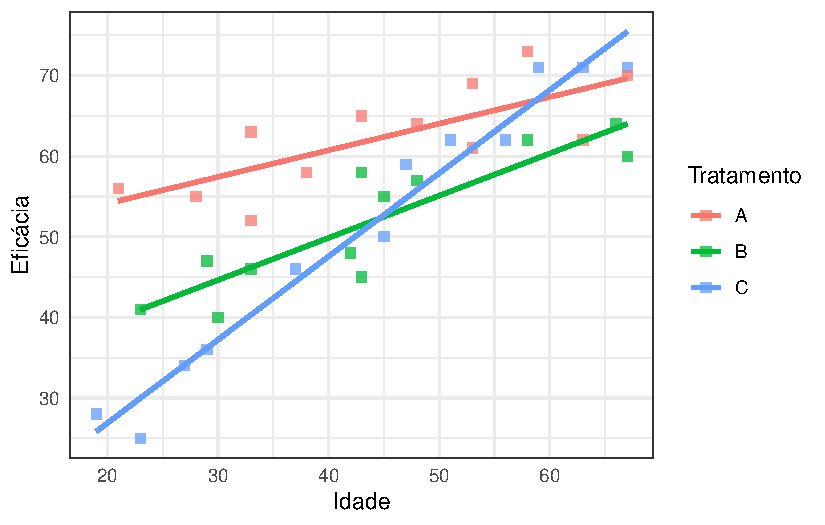
\includegraphics{lista2_files/figure-pdf/unnamed-chunk-1-1.pdf}

}

\caption{Curvas de regressão para modelo com interações.}

\end{figure}

Cabe recapitularmos que o grupo de referência é o tratamento C, o que
força a interpretação de que o intercepto \(\beta_0\) do modelo é o seu
efeito de tratamento isolado e \(\beta_1 \, x_{1i}\) se refere à
interação entre o tratamento C e a variável idade.

Enquanto este coeficiente, do grupo de referência, é positivo e muito
próximo a \(1\), os demais são negativos. No entanto, isto não significa
que suas retas têm coeficiente angular negativo. O sentido e magnitude
desses estimadores indica quanto a inclinação das demais retas está
deslocada no sentido horário em relação à referência. Pela tabela,
notamos que \(\beta_1 > \beta_4 > \beta_5\). Analogamente, se
\(\theta_j, j = A, B, C\) for o ângulo da curva de regressão em relação
às abscissas, notamos que \(\theta_C > \theta_B > \theta_A\).

Em termos reais, o modelo sugere que há uma grande influência da idade
sobre a eficácia do tratamento C, enquanto essa influência é menor para
o tratamento B e menor ainda para o tratamento A.

\hypertarget{iii-tabela-anova}{%
\subsubsection{iii) Tabela ANOVA}\label{iii-tabela-anova}}

Finalmente, montamos a tabela de ANOVA do modelo. Em contraposição ao
modelo anterior, sem interações, vemos que uma pequena parcela da soma
de quadrados é atribuída aos resíduos. De fato, o coeficiente associado
ao efeito puro do tratamento B ainda explica muito pouco da variação do
modelo. No entanto, para que possamos considerar a interação Idade
\(\times\) Tratamento B, que testa significativamente para
\(H_a: \beta_j \neq 0\), mantemos o efeito puro.

\begin{longtable}[t]{lccccl}
\caption{Tabela ANOVA para o modelo linear com interações}\\
\toprule
Fonte de Var. & g.l. & SQ & QM & F & p-valor\\
\midrule
\endfirsthead
\caption[]{Tabela ANOVA para o modelo linear com interações \textit{(continued)}}\\
\toprule
Fonte de Var. & g.l. & SQ & QM & F & p-valor\\
\midrule
\endhead

\endfoot
\bottomrule
\endlastfoot
\cellcolor{gray!15}{idade} & \cellcolor{gray!15}{1} & \cellcolor{gray!15}{3424.432} & \cellcolor{gray!15}{3424.432} & \cellcolor{gray!15}{222.295} & \cellcolor{gray!15}{0.000}\\
A & 1 & 803.804 & 803.804 & 52.178 & 0.000\\
\cellcolor{gray!15}{B} & \cellcolor{gray!15}{1} & \cellcolor{gray!15}{1.189} & \cellcolor{gray!15}{1.189} & \cellcolor{gray!15}{0.077} & \cellcolor{gray!15}{0.783}\\
idade:A & 1 & 375.002 & 375.002 & 24.343 & 0.000\\
\cellcolor{gray!15}{idade:B} & \cellcolor{gray!15}{1} & \cellcolor{gray!15}{328.424} & \cellcolor{gray!15}{328.424} & \cellcolor{gray!15}{21.319} & \cellcolor{gray!15}{0.000}\\
Residuals & 30 & 462.148 & 15.405 & NA & NA\\*
\end{longtable}

\hypertarget{iv-anuxe1lise-completa-dos-resuxedduos-do-modelo}{%
\subsubsection{iv) Análise completa dos resíduos do
modelo}\label{iv-anuxe1lise-completa-dos-resuxedduos-do-modelo}}

COMO?

Supõe-se que \(\varepsilon_i \sim N(0, \sigma^2)\).

\hypertarget{apuxeandice}{%
\section{Apêndice}\label{apuxeandice}}

Todo o projeto de composição deste documento pode ser encontrado aqui:
\url{https://github.com/cesar-galvao/mlg}



\end{document}
